\documentclass[12pt]{article}
\textwidth=17cm \oddsidemargin=-0.9cm \evensidemargin=-0.9cm
\textheight=23.7cm \topmargin=-1.7cm

\usepackage{amssymb, amsmath, amsfonts}
\usepackage{moreverb}
\usepackage{graphicx}
\usepackage{enumerate}
\usepackage{graphics}
\usepackage{color}
\usepackage{array}
\usepackage{float}
\usepackage{hyperref}
\usepackage{textcomp}
\usepackage{alltt}
\usepackage{physics}
\usepackage{mathtools}
\usepackage{tikz}
\usetikzlibrary{positioning}
\usetikzlibrary{arrows}
\usepackage{pgfplots}
\usepackage{bigints}
\usepackage[utf8]{inputenc}
\usepackage[english]{babel}
\usepackage{amsthm}
\usepackage{fancyhdr}
\usepackage[makeroom]{cancel}
\pagestyle{fancy}
\allowdisplaybreaks

\newcommand{\E}{\varepsilon}

\newcommand{\suchthat}{\, \mid \,}
\newcommand{\ol}[1]{\overline{#1}}
\newcommand{\bbar}[1]{\overline{#1}}
\newcommand{\inpd}[1]{{\left< \, #1 \, \right>}}
\renewcommand{\theenumi}{\alph{enumi}}
\newcommand\Wider[2][3em]{%
\makebox[\linewidth][c]{%
  \begin{minipage}{\dimexpr\textwidth+#1\relax}
  \raggedright#2
  \end{minipage}%
  }%
}

\def\R{\mathbb{R}}
\def\C{\mathbb{C}}
\def\H{\mathcal{H}}
\DeclareMathOperator*{\esssup}{\text{ess~sup}}
\newcommand{\resolv}[1]{\rho(#1)}
\newcommand{\spec}[1]{\sigma(#1)}
\newcommand{\iffR}{\noindent \underline{$\Longrightarrow$:} }
\newcommand{\iffL}{\noindent \underline{$\Longleftarrow$:} }
\newcommand{\lightning}{\textbf{\Huge \Lightning}}
\newcommand{\spt}[1]{\text{spt}(#1)}
\def\ran{\text{ ran}}
   
\newenvironment{myprob}[1]
    {%before text commands
    %{\Huge \_ \_ \_ \_ \_ \_ \_ \_ \_ \_ \_ \_ \_ \_ \_ \_ \_ \_ } \\
    \noindent{\Huge$\ulcorner$}\textbf{#1.}\begin{em}
    }
    { 
    %after text commands
    \end{em} \\ \hphantom{l} \hfill {\Huge$\lrcorner$} }
%	{\noindent \rule{7.5cm}{2pt} \textgoth{#1} \rule{8.cm}{2pt} \begin{em}}
%	{\end{em}\\ \vspace{0.1pt}\noindent \rule{\textwidth}{2pt}}
%
\setcounter{section}{-1}




\begin{document}
\lhead{MATH228A}
\chead{Carter Johnson - Homework 01}
\rhead{\today}

{\let\newpage\relax} 


%%%%%%%%%%%%%%%%%%%%%%%%%%%%%%%%%%%%%%%%%%%%%%%%%%%%% P1
\begin{myprob}{Problem 1}
Let $L$ be the linear operator $Lu = u_{xx}$, $u_x(0)=u_x(1)=0$.
\end{myprob}
%%%%%%%%%%%%%%% part a
\begin{enumerate}[ \ \ (a)]
\item Find the eigenfunctions and corresponding eigenvalues of $L$.
\end{enumerate}
\begin{align*}
u_{xx} - \lambda u = 0, u_x(0)=u_x(1)=0\\
\end{align*}
Assume $u= e^{kx}$, then the characteristic equation is $k^2 - \lambda = 0$, so $u = A e^{\sqrt{\lambda}x} + B e^{-\sqrt{\lambda}x}$.
Then $u_x = A\sqrt{\lambda} e^{\sqrt{\lambda}x} - B\sqrt{\lambda} e^{-\sqrt{\lambda}x}$,
so $u_x(0) = A\sqrt{\lambda} - B\sqrt{\lambda} = 0$
and $u_x(1)= A\sqrt{\lambda} e^{\sqrt{\lambda}} - B\sqrt{\lambda} e^{-\sqrt{\lambda}} = 0$.
The first boundary condition implies that $A=B$, then the second boundary condition is
$$A\sqrt{\lambda}\qty(e^{\sqrt{\lambda}}-e^{-\sqrt{\lambda}}) = 0.$$
This is only possible if $\lambda = 0$ or if $\lambda < 0$, in which case $$2A\sqrt{\lambda}\cos(\sqrt{\lambda})=0.$$
Thus for $\lambda<0$, we must have that $\lambda = -k^2 \pi^2$, $k>0$. \\

\noindent Thus we have our eigenvalues $\lambda_k = -k^2 \pi^2$ and eigenfunctions $u_k(x) = \cos(k\pi x)$, $k=0,1, \dots$.

%%%%%%%%%%%%%%% part b
\begin{enumerate}[ \ \ (b)]
\item Show that the eigenfunctions are orthogonal in the $L^2[0,1]$ inner product.
\end{enumerate}
Consider $u_n$ and $u_m$ eigenfunctions for $n\neq m$.
Then \begin{align*}
\inpd{u_n, u_m} &= \int_0^1 \cos(n \pi x) \cos(m \pi x) \dd x \\
&= \frac{1}{2}\int_0^1 \cos( (n+m) \pi x) + \cos((n-m)\pi x) \dd x \\
&= \frac{1}{2} \qty[ -\frac{1}{(n+m)\pi} \sin((n+m)\pi x) - \frac{1}{(n-m)\pi} \sin((n-m)\pi x)  ]_0^1 \\
&= 0.
\end{align*}
Where the last equality holds because $n+m$ and $n-m$ are both integers, and $\sin$ of any integer multiple of $\pi$ is $0$.

For $n=m$, then \begin{align*}
\inpd{u_n, u_m} &= \int_0^1 \cos^2(n \pi x)\dd x \\
&= \frac{1}{2}\int_0^1 1+\cos(2n\pi x) \dd x \\
&= \frac{1}{2} \qty[ x -\frac{1}{2n\pi} \sin(2n\pi x)]_0^1 \\
&= \frac{1}{2}.
\end{align*}

%%%%%%%%%%%%%%% part c
\begin{enumerate}[ \ \ (c)]
\item It can be shown that the eigenfunctions $\phi_j(x)$, form a complete set in $L^2[0,1]$. Express the solution to $$u_{xx} = f, u_x(0)=u_x(1) = 0,$$ as a series solution of the eigenfunctions.
\end{enumerate}
Since the eigenfunctions form a complete set, we can express $f$ as series
\begin{align*}
f(x) &= \sum_{j=0}^\infty f_j \phi_j(x).
\end{align*}
where $$f_j = \dfrac{\inpd{f, \phi_j}}{ \inpd{\phi_j, \phi_j}}.$$
Then assuming the solution has the form $$u(x) = \sum_{j=0}^\infty a_j \phi_j(x),$$
we have that 
\begin{align*}
u_{xx} &= f \\
\sum_{j=0}^\infty \lambda_j a_j \phi_j(x) &= \sum_{j=0}^\infty f_j \phi_j(x).
\end{align*}
If we take the inner product of the above equation with any $\phi_j$, by orthogonality we will obtain the single terms
$$\lambda_j a_j \inpd{\phi_j, \phi_j} = f_j \inpd{\phi_j, \phi_j}.$$
Thus $$a_j = \dfrac{f_j}{\lambda_j} = \dfrac{\inpd{f, \phi_j}}{ -j^2\pi^2 \inpd{\phi_j, \phi_j}},$$
so that $$u(x) = \sum_{j=0}^\infty  \dfrac{\inpd{f, \phi_j}}{ -j^2\pi^2 \inpd{\phi_j, \phi_j}} \phi_j(x).$$

%%%%%%%%%%%%%%% part d
\begin{enumerate}[ \ \ (d)]
\item Note that the BVP does not have a solution for all $f$.  Express the condition for existence of a solution in terms of the eigenfunctions of $L$.
\end{enumerate}

In order for $Lu = f$ to have a solution, $f$ must be in the range of $L$.  Since $$L^2[0,1] = \ran{L} \bigoplus \ker{L^*},$$ $f$ must be orthogonal to $\ker{L^*}$.  Since $L$ is self-adjoint, $f$ must be orthogonal to $\ker{L}$.  Note that $\ker{L}$ is spanned by $\phi_0(x) = 1$, since $\phi_0(x)$ has eigenvalue $0$.  Thus 
$$\inpd{f,\phi_0} = \inpd{f,1} = \int_0^1 f(x) \dd x = 0.$$


%%%%%%%%%%%%%%%%%%%%%%%%%%%%%%%%%%%%%%%%%%%%%%%%%%%%% P2
\begin{myprob}{Problem 2}
Define the functional $F: X \to \R$ by
$$F(u) = \int_0^1 \dfrac{1}{2}(u_x)^2 + fu \dd x,$$
where $X$ is the space of real valued functions on $[0,1]$ that have at least one continuous derivative and are zero at $x=0,1$.  The Frechet derivative of $F$ at a point $u$ is defined to be the linear operator $F'(u)$ for which $$F(u+v) = F(u)+F'(u)v + R(v),$$
where $$\lim_{\norm{v}\to0} \dfrac{ \norm{R(v)}}{\norm{v}} = 0.$$
One way to compute the derivative is $$F'(u)v = \lim_{\E \to 0} \dfrac{F(u+\E v)-F(u)}{\E}.$$
Note that this looks just like a directional derivative.
\end{myprob}
%%%%%%%%%%%%%%% part a
\begin{enumerate}[ \ \ (a)]
\item Compute the Frechet derivative of $F$.
\end{enumerate}

\begin{align*}
F'(u)v &= \lim_{\E\to0}\dfrac{1}{\E} \int_0^1 \dfrac{1}{2}(u_x + \E v_x)^2 + f(u+\E v) - \dfrac{1}{2}(u_x)^2 - fu \dd x \\
&= \lim_{\E\to0} \dfrac{1}{\E} \int_0^1 \E u_x v_x + \dfrac{1}{2}\E^2 v_x^2 + \E f v \dd x \\
&= \int_0^1 u_x v_x + f v \dd x \\
&= \cancelto{0}{[u_x v]_0^1} + \int_0^1 fv - u_{xx}v \ \dd x \ \ \text{by $v \in X$} \\
&= \int_0^1 (f - u_{xx}) v \ \dd x.
\end{align*} 

%%%%%%%%%%%%%%% part b
\begin{enumerate}[ \ \ (b)]
\item $u \in X$ is a critical point of $F$ if $F'(u)v = 0$
for all $v \in X$. Show that if $u$ is a solution to
the Poisson equation
$$u_{xx} = f, u(0) = u(1) = 0,$$
then it is a critical point of $F$.
\end{enumerate}

If $u$ solves $$u_{xx} = f, u(0) = u(1) = 0,$$ then for all $v \in X$,
$$F'(u)v = \int_0^1 (f-u_{xx})v \ \dd x = \int_0^1 0 v \ \dd x = 0.$$
Hence $u$ is a critical point of $F$.

%%%%%%%%%%%%%%% part c
\begin{enumerate}[ \ \ (c)]
\item   Let $X_h$ be a finite dimensional subspace of $X$, and let $\{\phi_i(x)\}$ be a basis for $X_h$.  This means that all $u_h \in X_h$ can be expressed as $u_h(x) = \sum_iu_i\phi_i(x)$ for some constants $u_i$.  Thus we can identify the elements of $X_h$ with vectors $\vec{u}$ that have components $u_i$.  Let $G(\vec{u}) = F(u_h)$.  Show that the gradient of $G$ (whos components are $(\grad G)_j = \frac{\partial G}{\partial u_j})$ is of the form $\grad G(\vec{u}) = A\vec{u} + \vec{b}$, and write expressions for the elements of the matrix $A$ and the vector $\vec{b}$.
\end{enumerate}

\begin{align*}
F(u_h) &= \int_0^1 \dfrac{1}{2}(u_{h,x}^2 + fu) \ \dd x \\
G(\vec{u}) &= \int_0^1 \dfrac{1}{2} \qty(\sum_i u_i \phi_i')^2 + f(\vec{u}\cdot\vec{\phi}) \ \dd x \\
\implies \dfrac{\partial G}{\partial u_j}(\vec{u}) &= \int_0^1 \phi_j'(\vec{u}\cdot\vec{\phi}') + f \phi_j  \ \dd x \\
&= \qty[(\vec{u}\cdot\vec{\phi}')\phi_j]_0^1 + \int_0^1 (f- \dfrac{\dd }{\dd x}(\vec{u}\cdot\vec{\phi}'))\phi_j \ \dd x\\
&= \int_0^1 \qty[f- \vec{u}\cdot\vec{\phi''} ]\phi_j \ \dd x,
\end{align*}
where the boundary terms vanish since $\phi_j \in X$.

This can be represented as
$$\nabla G (\vec{u}) = A\vec{u} + \vec{b},$$
where $$(A)_{ij} = - \int_0^1 \phi_i \phi_j'' \ \dd x$$
and $$(\vec{b})_j = \int_0^1 f \phi_j \ \dd x.$$
%%%%%%%%%%%%%%% part d
\begin{enumerate}[ \ \ (d)]
\item    Divide the unit interval into a set of $N+1$ equal length intervals $I_i = (x_i,x_{i+1})$ for $i = 0, \dots, N$.  The enpoints of the intervals are $x_i = ih$, where $h = \frac{1}{N+1}$.  Let $X_h$ be the subspace of $X$ such that the elements $u_h$ of $X_h$ are linear on each interval, continuous on $[0,1]$, and satisfy $u_h(0) = u_h(1) = 0$.  $X_h$ is an $N$ dimensional space with basis elements
    \begin{align}
        \phi_i(x) = \begin{cases}
            1 - h^{-1}\abs{x - x_i} & \text{ if } \abs{x - x_i} < h,\\
            0 & \text{ otherwise}
        \end{cases}
    \end{align}
    for $i = 1, \dots, N$.  Compute the matrix $A$ from the previous problem that appears in the gradient.
\end{enumerate}

Note that $$\phi_i ' = \begin{cases}
  1/h, & x_{i-1} < x < x_i \\ -1/h, & x_i < x < x_{i+1} \\ 0, & \text{o/w}. \end{cases}$$
So that $$\phi_i'' = \delta(x-x_i).$$
Then $$(A)_{ij} = - \int_0^1 \phi_i(x)\phi_j''(x) \ \dd x = \int_0^1 \phi_i(x) \delta(x-x_j) \ \dd x= -\phi_i(x_j).$$
Thus $(A)_{ij} = 0$ for $j\neq i$, and $(A)_{ii} = -1$, so $A = -I$. 

%%%%%%%%%%%%%%%%%%%%%%%%%%%%%%%%%%%%%%%%%%%%%%%%%%%%% P3
\begin{myprob}{Problem 3}
\end{myprob}
%%%%%%%%%%%%%%% part a
\begin{enumerate}[ \ \ (a)]
\item Using a Taylor expansion, derive the finite difference formula to approximate the second derivative at $x$ using function values at $x - \frac{h}{2}$, $x$, and $x + h$.  How accurate is the finite difference approximation?
\end{enumerate}

We begin by Taylor expanding $u(x-\dfrac{h}{2})$ and $u(x+h)$.
$$u(x-\dfrac{h}{2}) = u(x) - \dfrac{h}{2}u'(x) + \dfrac{h^2}{8}u''(x) -\dfrac{h^3}{48} u'''(x) + \dots \ .$$
$$u(x+h) = u(x) + h u'(x) + \dfrac{h^2}{2} u''(x) + \dfrac{h^3}{6}u'''(x)+\dots \ .$$
Then clearly, 
$$u(x-\dfrac{h}{2}) + \dfrac{1}{2}u(x+h) = \dfrac{3}{2}u(x)  + u''(x)\qty(\dfrac{h^2}{8}+\dfrac{h^2}{4}) +u'''(x)\qty(\dfrac{h^3}{12} + \dfrac{h^3}{48}) + \dots \ .$$
So $$u(x-\dfrac{h}{2}) + \dfrac{1}{2}u(x+h)  - \dfrac{3}{2}u(x) = \dfrac{3h^2}{8}u''(x) + \dfrac{3h^3}{48}u'''(x)+ \dots \ .$$
Let $$Du = \dfrac{4}{3h^2}\qty[2 u(x-\dfrac{h}{2}) - 3u(x) + u(x+h)].$$
Then this is a first-order accurate approximation of $u''(x)$ with error $$Du - u''(x) = \dfrac{8h}{48}u'''(x) + \dots = \order{h}.$$
%%%%%%%%%%%%%%% part b
\begin{enumerate}[ \ \ (b)]
    \item Perform a refinement study to verify the accuracy of the difference formula you derived.
    \end{enumerate}

I applied this difference formula to the function $u(x) = \dfrac{x^3}{3}$ at $x=10$ for various grid spacings $h$, and plotted the errors of our approximation on a log-log plot against the grid spacing.
\begin{figure}[H]
\centering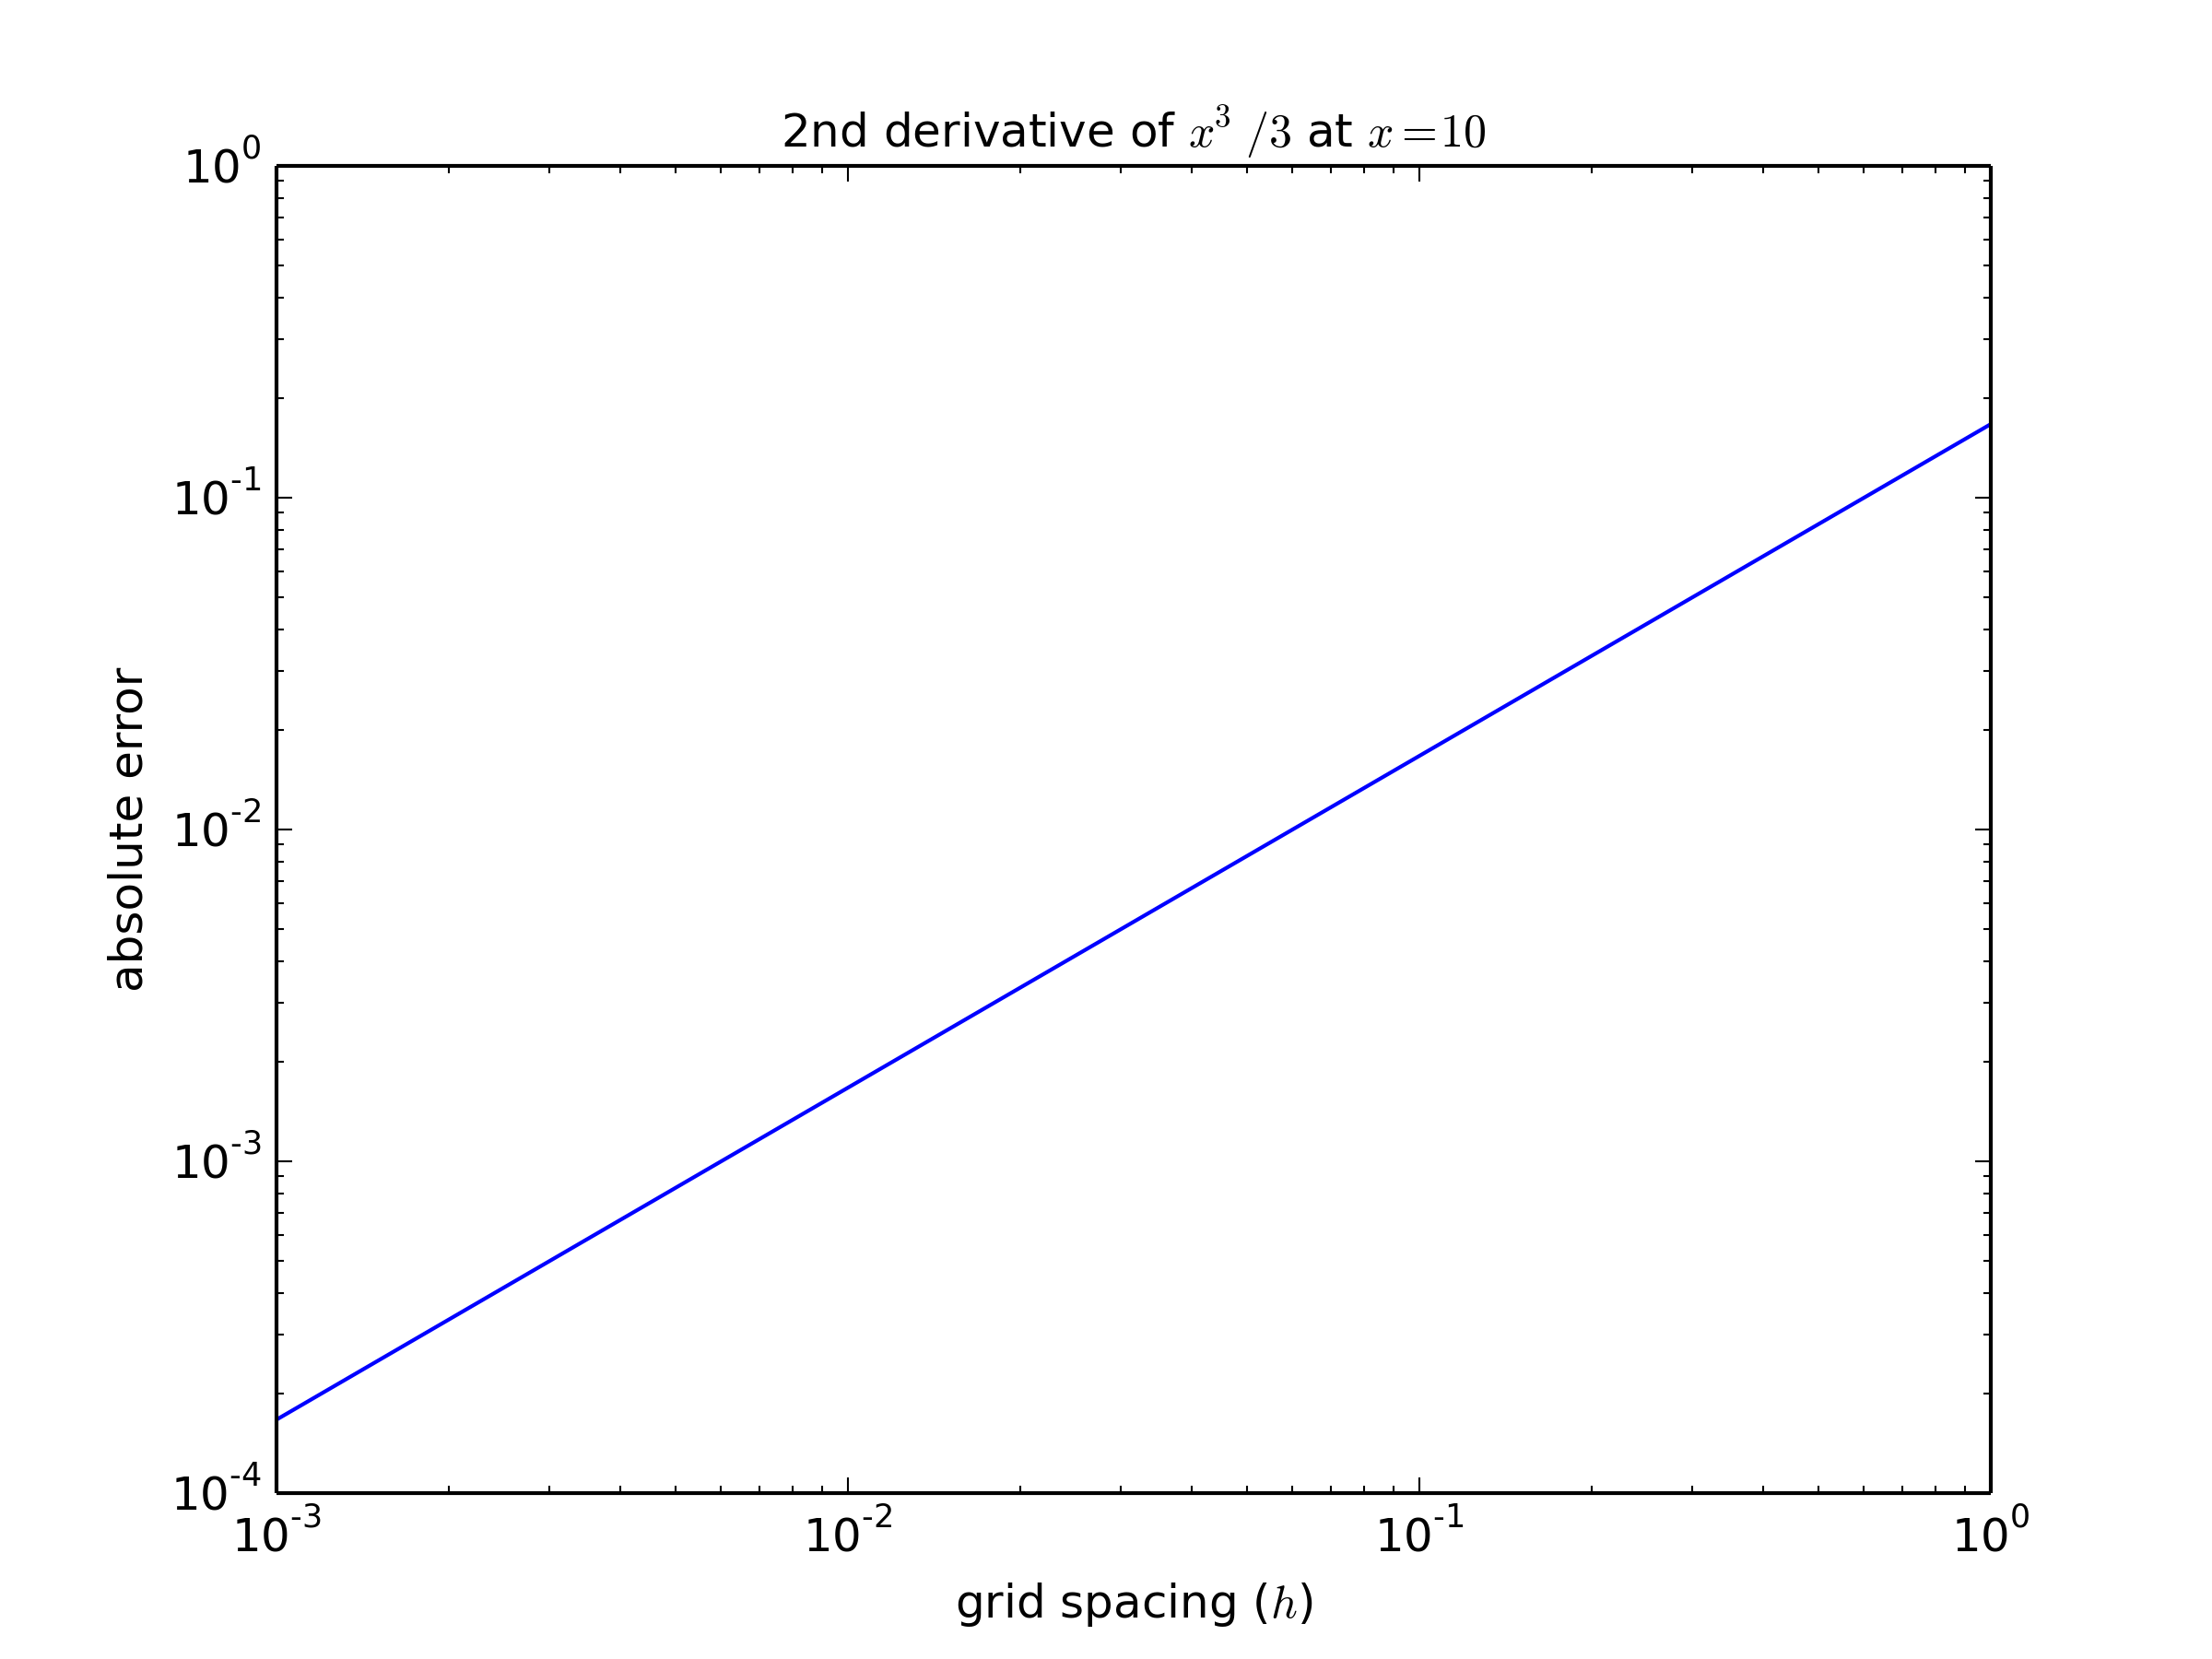
\includegraphics[scale=0.75]{problem3_refinement_study.png}
\end{figure}
Note that the slope appears to be $1$, so this is indeed a first-order accurate approximation of $u''(x)$.

%%%%%%%%%%%%%%% part c
\begin{enumerate}[ \ \ (c)]
    \item Derive an expression for the quadratic polynomial that interpolates the data $\qty(x - \frac{h}{2}, u\qty(x - \frac{h}{2}))$, $(x, u(x))$, and $(x + h, u(x + h))$.  How is the finite difference formula you derived in problem 3a related to the interpolating polynomial?
    \end{enumerate}
We want to find a polynomial $u(x) = A + Bx + Cx^2$ interpolating these points. With $u_0 = u(x-\dfrac{h}{2})$, $u_1 = u(x)$, $u_2 = u(x+h)$,
we solve the system of equations 
\begin{align*}
u_0 &= A + B(x-\dfrac{h}{2}) + C(x-\dfrac{h}{2})^2 \\
u_1 &= A + Bx + Cx \\
u_2 &= A + B(x+h) + C(x+h)^2
\end{align*}
using Maple to obtain:
    $$A={\frac {3\,{\it u_1}\,{h}^{2}+4\,{\it u_0}\,xh-3\,{\it u_1}\,xh-{\it u_2}\,
xh+4\,{\it u_0}\,{x}^{2}-6\,{\it u_1}\,{x}^{2}+2\,{\it u_2}\,{x}^{2}}{3{h}^{2}}},$$ $$B=-
{\frac {4\,h{\it u_0}-3\,h{\it u_1}-h{\it u_2}+8\,{\it u_0}\,x-12\,{\it u_1}\,x+
4\,{\it u_2}\,x}{3{h}^{2}}}$$
$$C = \dfrac{2}{3h^2}\qty(2u_0-3u_1 + u_2).$$

Note that if we take the second derivative of this interpolating polynomial, we obtain 
$$u''(x) = 2C = \dfrac{4}{3h^2}\qty(2u_0-3u_1 + u_2) = Du.$$

So we have found a second way to construct our difference approximation operator. \\

\noindent \textbf{Python Code used for 3b:}
\begin{verbatim}
#hw_01_228A Refinement Study (problem 3 part b)
#Carter Johnson
#10/11/16

import numpy as np
from math import exp
import matplotlib.pyplot as plt

#my problem is x^3/3 -> second derivative is x
#evaluate at x=10
x=10
actual = 10

#2nd derivative approximate operator as function of grid spacing h
def D2_approx(h):
  return (2/(3*h**2))*(2*(x-h/2)**3/3 + (x+h)**3/3 - (x)**3)

#evaluate my 2nd derivative approximation for various h 
H = np.linspace(1, .001, 100)
D2_approxes = [D2_approx(h) for h in H]

#find abs errors of these approximations
max_errors = [abs(approx - actual) for approx in D2_approxes]

#plot as log-log
plt.figure()
plt.loglog(H, max_errors, label="Absolute Error")
plt.title("2nd derivative of $x^3/3$ at $x=10$", fontsize=12)
plt.xlabel("grid spacing ($h$)")
plt.ylabel("absolute error")
plt.savefig("problem3_refinement_study.png", dpi=300)
plt.close()
\end{verbatim}
%%%%%%%%%%%%%%%%%%%%%%%%%%%%%%%%%%%%%%%%%%%%% end
\end{document}